\newpage
%\chapter{Descripción} \label{cap:Herramienta SLAMTestbed}
\chapter{Herramienta SLAMTestbed} \label{cap:Herramienta SLAMTestbed} %chapter 4
%\setcounter{section}{4}
En este capítulo se detalla el diseño y la implementación de SLAMTestbed, una aplicación diseñada y creada para comparar cuantitativamente algoritmos SLAM. El diseño de algoritmos SLAM, y de Visual SLAM en particular es todavía una disciplina abierta en expansión y cuenta cada vez con un mayor número de aplicaciones reales, entre las que destaca la navegación de vehículos autónomos o las aplicaciones de realidad aumentada. Existe un gran número de algoritmos SLAM, por lo que se necesitan herramientas que  permitan medir su precisión, robustez y velocidad de cada algoritmo.

Comenzaremos explicando el diseño de la herramienta SLAMTestbed desde un punto de vista de caja negra, explicando sus entradas y sus salidas. Se continuará con la explicación de su diagrama de bloques y se finalizará profundizando en cada uno de los bloques principales de la herramienta es decir, los distintos módulos que permiten calcular el Registro Espacial ( Escala, Traslación y Rotación) y el Registro Temporal (interpolación de frecuencias y cálculo de \textit{Offset} o Desplazamiento Temporal) entre dos secuencias de posiciones y orientaciones 3D.

\section{Diseño}

En esta sección no entraremos en los detalles de la implementación de la herramienta SLAMTestbed, si no que lo trataremos como una \textit{caja negra}.
En la entrada del sistema tendremos dos secuencias de puntos 3D orientados.
Las secuencias procesadas por esta herramienta serán ficheros de texto cuyos registros tendrán los siguientes 8 campos:

\textit{Timestamp, X, Y, Z, qx,qy,qz,qw}

Uno de los \textit{datasets} será la verdad absoluta, y el segundo \textit{dataset} será la posición y orientación en 3D obtenidos tras aplicar un algoritmo Visual SLAM, correspondiendo cada registro del \textit{dataset} con una posición de la cámara.
Una vez procesados los dos \textit{datasets} por SlamTestbed, obtendremos como salida las transformaciones estimadas por la herramientas entre la verdad absoluta y las posiciones y orientaciones calculadas por el algoritmo de SLAM. Además, se obtendrá un conjunto de estadísticos que miden el error cometido en las estimaciones de SLAM y así caracteriza la precisión de los algoritmos.


\begin{figure}[H]
\begin{center}
\label{fig:Open File}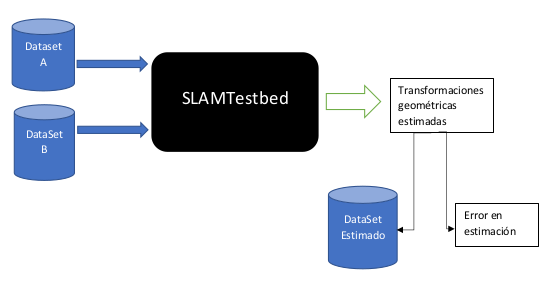
\includegraphics[height=8.0cm,width=14.0cm]{img/cap5/Esquema_TFM_CajaNegra2.png}
\hspace{0.5cm}
%\subfigure[]{\label{fig:LG_hombot}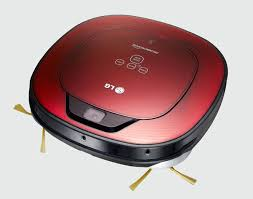
\includegraphics[height=6.0cm]{img/cap2/LG_hombot.jpg}}
\end{center}
%\caption{Robot Dyson 360 Eye (a) Robot Roomba 966 (b) Robot Hombot de LG (c).}
\caption{ El diseño de caja negra de la herramienta SLAMTestbed. }
\end{figure}

%\section{Diseño de caja Blanca}
Una vez explicadas las entradas y salidas de la aplicación ahora explicaremos
con más detalle la implementación de la herramienta SLAMTestbed. El objetivo principal de la herramienta desarrollada es calcular el error existente entre una secuencia con las posiciones y orientaciones 3D verdaderas (\textit{dataset A}) y la trayectoria calculada por el algoritmo de SLAM (\textit{dataSet B}). Para que esto sea posible necesitaremos antes eliminar algunas variables que no permiten comparar directamente las dos trayectorias, como son la escala, el \textit{offset} temporal y la transformación en 3D entre ellas. Por ello, necesitaremos calcular un nuevo \textit{dataset} (estimado), que sea comparable con el \textit{dataset A}. 

Las principales funciones o módulos utilizados para obtener el \textit{dataset} estimado son:

\begin{description}
\item [Cálculo de PCA]:

El análisis de componentes principales (o PCA), permite reducir los dos  \textit{dataSets} a sus componentes principales, lo que posibilita estimar a continuación la escala y el offset existente entre ellos.
\item [Estimación de Escala]: 

Estima la diferencia de escala entre los dos \textit{datasets} a partir de los datos proporcionados en el cálculo de componentes principales.
\item [Estimación de Offset temporal]: 

Con este módulo podremos hallar la diferencia entre marcas de tiempos de los 2 \textit{datasets}, ya que pueden haber comenzado en periodos de tiempo distintos.
\item [Interpolación para igualar frecuencias de muestreo]: 

Con la interpolación podremos igualar en frecuencia los dos \textit{datasets}, en caso de que éstas sean distintas, que es lo habitual por que el algoritmo SLAM genera estimaciones a diferente ritmo del que vienen las muestras de la secuencia con verdad absoluta.

\item [Operaciones de Registro para estimar la Rotación y Traslación]: 

Permite estimar la traslación y rotación existentes entre el \textit{dataset A} y el \textit{dataset B} y llevarlas así al mismo sistema de referencia espacial, donde ya son directamente comparables.
\end{description}


%\begin{figure}[H]
\begin{figure}
\begin{center}
\label{fig:Open File}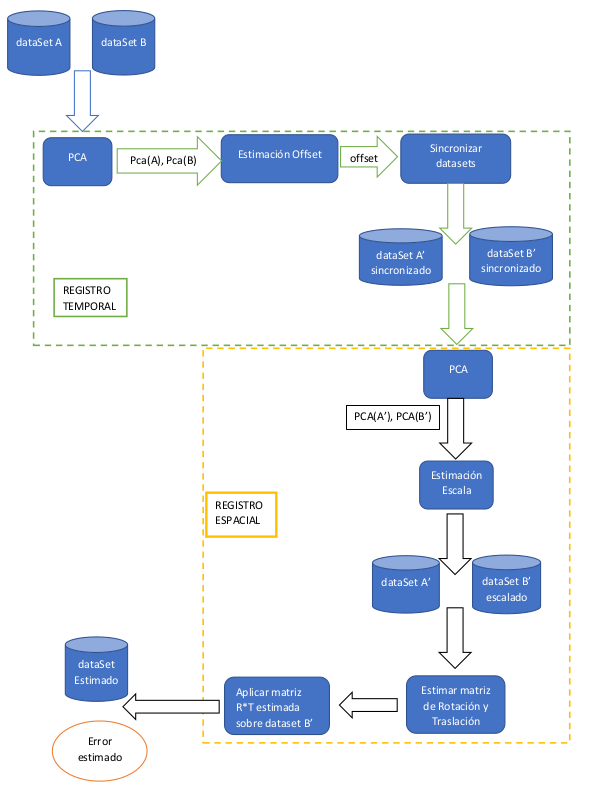
\includegraphics[height=18.0cm,width=12.0cm]{img/cap5/EsquemaTFM_CajaBlanca_Transformaciones4.png}
\hspace{0.5cm}
%\subfigure[]{\label{fig:LG_hombot}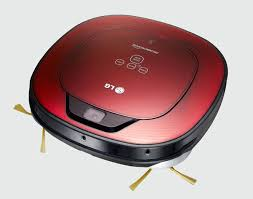
\includegraphics[height=6.0cm]{img/cap2/LG_hombot.jpg}}
\end{center}
%\caption{Robot Dyson 360 Eye (a) Robot Roomba 966 (b) Robot Hombot de LG (c).}
\caption{ Diagrama de bloques de la herramienta SLAMTestbed }
\end{figure}

La explicación al flujo de datos seguido en la Figura 4.2 es el siguiente: Primero se calcula la descomposición en componentes principales (PCA) para cada uno de los \textit{datasets} obteniendo como resultado \textit{dataSet A'} y \textit{dataSet B'}. Posteriormente se estima el \textit{offset} o desplazamiento de tiempo que existe entre las 2 secuencias de datos o \textit{datasets}. Corrigiendo el offset en el \textit{dataset B}, sumando el valor del \textit{offset} calculado a los valores de tiempo del \textit{dataset B} así las dos secuencias tienen ya el mismo origen de tiempos. Una vez tengamos calculado el offset, unificaremos las frecuencias de los 2 \textit{datasets} mediante interpolación. En este proceso de interpolación se generarán nuevas muestras para los \textit{datasets'}.
Cuando tengamos unificada la frecuencia para los dos \textit{datasets}, obtendremos de nuevo PCA de ambos \textit{datasets} y podremos obtener la escala entre ambos.
Posteriormente estimaremos la transformaciones de rotación y traslación para pasar del \textit{dataset A} al \textit{dataset B}. Aplicaremos dichas transformaciones sobre el \textit{dataset A}, para obtener un nuevo \textit{dataset}, el \textit{dataset} Estimado que pintaremos en pantalla de color rojo.

En las siguientes secciones se explicarán con más detalle cada uno de estos módulos.


\section{Estimador PCA y Cálculo de Escala}
    El análisis de componentes principales (\textit{PCA} según sus siglas en inglés) es el algoritmo más utilizado para reducir las dimensiones de un conjunto de datos. Como resultado de aplicar PCA sobre un conjunto de datos, obtendremos un nuevo conjunto de datos en términos de nuevas variables no correlacionadas, que denominaremos componentes principales.

    Las componentes principales se ordenarán por su Varianza, de esta forma la primera componente principal será la que mayor varianza tenga e identificará un eje. Un segundo eje ortogonal al primero vendrá definido por la segunda componente principal e identificará la segunda mayor varianza. Finalmente obtendremos un tercer eje ortogonal a los dos primeros, definido por la tercera componente principal que identificará la tercera mayor varianza.

    En nuestro caso, este análisis permitirá obtener el tamaño de cada \textit{dataset} en cada una de sus componentes (x,y,z)
	Este análisis es necesario puesto que los ejes de las dos secuencias de entrada no tienen porqué coincidir. Por ello, con los valores obtenidos con PCA podremos generar dos nuevos \textit{datasets} cuyos ejes sean comparables, es decir que estén alineados. A partir de los nuevos \textit{datasets} generados podremos calcular la diferencia de tiempos entre los dos \textit{datasets} y posteriormente la escala entre ambos.
 
	Se implementan dos métodos de cálculo de PCA, el primero es realizando una descomposición Eigen \textit{eigenDecomposition}, el segundo utilizando el método SVD (utilizando la librería Eigen), que describiremos a continuación en pseudocódigo.

	\begin{lstlisting}[frame=single]
		# Obtener el valor medio de cada componente
		mX = media (dataset.x)
		mY = media (dataset.y)
		mZ = media (dataset.z)

		#restar la media a cada componente x, y z

		dataset2.x = dataset.x - mX
		dataset2.y = dataset.y - mY
		dataset2.z = dataset.z - mZ
        
        #Calcular el nuevo dataset

		cov = obtenerMatrizCovarianza(dataset2)
		svd = CalularSVD(cov )
		pca =  Matriz V del resultado svd
		datasetResultado = dataset * Matriz (svd.V)

	\end{lstlisting}

    Una vez que los ejes de ambos \textit{datasets} sean comparables, podremos calcular la diferencia de escala entre los dos \textit{datasets}, lo que permitirá igualar la escala entre los \textit{datasets} obteniendo así el primer paso del registro espacial. El algoritmo utilizado está basado en la utilización de los valores singulares de cada \textit{dataset}, como se muestra en el siguiente pseudocódigo:

        
	\begin{lstlisting}[frame=single]
		S1 = svd(dataSet1).valoresSingulares
		S2 = svd(dataSet2).valoresSingulares
		scalaX = S2(0)  / S1(0)
		scalaY = S2(1)  / S1(1)
		scalaZ = S2(2)  / S1(2)
	\end{lstlisting}

	En este caso asociamos al eje X la componente con mayor varianza, al eje Y el segunda componente con mayor varianza y al eje Z la tercera componente de mayor varianza. Pero en ocasiones esta correspondencia no es la conveniente y al usuario se le debe permitir realizar la asociación adecuada entre los ejes X,Y,Z y las 3 componentes principales.




\section{Estimador Offset Temporal}

Este módulo es necesario puesto que los \textit{datasets} pueden tener un desfase en su inicio, incluso aunque hayan sido obtenidos a partir de la misma secuencia, debido a la propia implementación de los algoritmos SLAM. El método principal utilizado para estimar el offset se realiza mediante el cálculo de la Correlación Cruzada. 
Este método conlleva una gran carga para la CPU ya que incluye múltiples cálculos para interpolar y calcular la correlación cruzada entre los dos \textit{datasets}. Este algoritmo es iterativo y utilizaremos un dataset como base de tiempo fijo y otro dataset B que se deslizará en el tiempo desde -T hasta +T en pequeños incrementos de tiempo, pasos o \textit{steps} en cada iteración, calculando para cada paso la correlación cruzada entre el \textit{dataset} deslizante y el \textit{dataset} original (que se mantiene fijo en el tiempo).

En cada iteración del algoritmo se calculará la correlación para un paso determinado, almacenando la memoria el paso cuya correlación sea mayor, lo que nos indicará el offset temporal estimado entre las dos secuencias. Para ello calcularemos la interpolación para los puntos 3D orientados que estén dentro del rango temporal de los dos \textit{datasets}. Una vez interpolados los puntos 3D comunes de las dos series temporales tendremos dos series nuevas, para las cuales calcularemos la correlación cruzada aplicando el algoritmo clásico para dos series temporales. Pero antes, y como cada serie temporal tiene 3 coordenadas (x,y,z para cada punto 3d), debemos transformar estas 3 coordenadas en un sólo valor para cada punto 3D de cada serie. Para ello tendremos que calcular la distancia al origen de todo punto 3D, y por tanto la correlación cruzada se calculará sobre los dos \textit{datasets} convertidos a distancias al origen de coordenadas.
Para un punto 3d (x,y,z), la distancia 3d respecto al origen se calculará:
\begin{center}
	\begin{math}
	\sqrt{(x-0)^2 +(y-0)^2+(z-0)^2}
	\end{math}
\end{center}

\begin{figure}[H]
\begin{center}
\label{fig:opciones de View}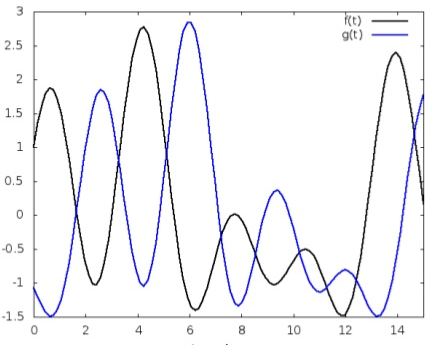
\includegraphics[height=8.0cm,width=12.0cm]{img/cap5/correlacionCruzada2.png}
\hspace{0.5cm}

\end{center}

\caption{Desfase del offset entre dos series temporales.}
\end{figure}
	                                
	\begin{lstlisting}[frame=single]
	dataA(d) = CalcularDistanciaAlOrigen( dataSetA(x,y,z))
	dataB(d) = CalcularDistanciaAlOrigen( dataSetB(x,y,z))
	mA = CalcularMedia(dataA)
	mB = CalularMedia(dataB)

	Para cada fila

   		sx = dataA(i) - mA

   		sy = dataB(i) - mB

   	denom = sqrt(sx*sy);
   	step = 0.01
   	Desde i=-T hasta i = T
   		Si ( dataB.t < dataB.t )
			j=j+1
    		continuar

    	sino si (dataB.t > dataA.t)
    		i=i+1
    		continuar

    	sino si (dataB.t == dataA.t)
    		sxy=(dataA -mA) * (dataB-mB)
        	i++
        	j++


   

   r = (sxy) / denom;

   r= fabs(r);
    \end{lstlisting}



\section{Interpolador temporal}

	El módulo de interpolación se utiliza para sincronizar a igual frecuencia 2 secuencias, cuyas frecuencias de muestreo no sean iguales, algo que es común entre los algoritmos de SLAM.
	En este proceso de interpolación se generarán nuevos puntos 3D orientados en el \textit{dataset} a partir de la interpolación de muestras entre dos marcas de tiempo.
	Este interpolador puede configurarse para que tenga distintos comportamientos:
    \begin{enumerate}
	 
	 \item{\textbf{Interpolación a la frecuencia menor}} de los dos \textit{datasets}. Aunque se generarán nuevos registros sincronizados por interpolación, en general se perderán registros del dataset de mayor frecuencia.

	 \item{\textbf{Interpolación a la frecuencia mayor}} de los dos \textit{datasets}. En este caso se generarán nuevos registros para el dataset de menor frecuencia.

	 \item{\textbf{Interpolación a frecuencia común}}, en este caso, los dos \textit{datasets} se deberán sincronizar a la frecuencia deseada por el usuario.
	 \end{enumerate}

	 En los tres casos, la interpolación se realiza sobre las secuencias temporales de los 2 \textit{datasets}, pero además se calcula la interpolación para las coordenadas X,Y,Z de cada punto 3D y valores (qx,qy,qz,qw) de cada cuaternio. La función \textit{slerp} de la librería Eigen permite calcular la interpolación entre cuaternios, viene de la abreviatura de la definición en inglés \textit{Spherical Linear intERPolation}, creada para animaciones de rotaciones 3D utilizando cuaternios.


	 La fórmula para la interpolación lineal utilizada sería:

	 \begin{center}
	 \begin{math}
		y-y2= (t-t2)*\frac{y3-y2}{t3-t2}
	 \end{math}
	 \end{center}

	 Donde t sería el nuevo valor de tiempo para el cual deberíamos interpolar los nuevos valores de las cordenadas X,Y,Z. 
	 Los valores t3,y3 hacen referencia al valor de la secuencia en t+1
	 Los valores t2,y2 hacen referencia al valor de la secuencia en t-1

	 %double y= y2 + (x-x2)*((y3-y2)/(x3-x2));
	 %double y2= (B.row(contB-1))(1);
	%double x = (A.row(contA-1))(0);t
	%double x2= (B.row(contB-1))(0);t2
	%double y3= (B.row(contB))(1);
	%double x3= (B.row(contB))(0);t3
	 



\section{Registro Espacial}
Una vez modificados los dos \textit{datasets} para que tengan la misma escala y la misma frecuencia de muestreo y el mismo origen temporal, el siguiente paso es obtener la rotación y la traslación 3D que existe entre ellos. Esta matriz servirá para transformar el segundo \textit{dataset}, y así poder calcular el error existente en la trayectoria obtenida por el algoritmo de SLAM.
Los pasos necesarios para realizar este registro espacial son los siguientes:

\textbf{Hallar la matrices de rotación y traslación} .

	\begin{lstlisting}[frame=single]
    # Hallar los centroides para las coordenadas X,Y,Z 
    	centA = centroides (A)
    	centB = centroides (B)
    

    # Restar los centroides a sus respectivas matrices
      	A= A-centA
      	B= B-centB
    
    # Calcular el producto de las matrices
    	H = A.traspuesta * B

    # Obtener valores singulares de la matriz H
    	S,U,V = svd(H)
    
    # Obtener la matriz de Rotacion
      	R = V*U.traspuesta

    # Obtener la matriz de Traslacion
    	t= -R * centA + centB;  
    \end{lstlisting}

\textbf{Transformar un \textit{dataset} aplicando las matrices de Rotación y Traslación estimadas}

Este método tomará un \textit{dataset}, lo multiplicará por la matriz de rotación y le sumará la matriz de traslación.

\textbf{Transformar los cuaternios aplicando la matriz Rotación.}

Con este método conseguimos transformar los cuaternios del \textit{dataSet A} al \textit{dataSet B}. Para ello convertiremos la matriz de rotación en un cuaternio que llamaremos "q". Por último multiplicaremos cada cuaternio p de la siguiente forma.
\begin{center}
		\textit{q * p * q.inverso }
\end{center}

\textbf{Estimar las matrices de rotación y traslación mediante la técnica de RANSAC.}
Estimaremos las matrices de Rotación y Traslación utilizando los datos de los dos \textit{datasets}, eliminando primero los puntos espurios \textit{outliers}) mediante el algoritmo RANSAC \cite{Fischler:1981:RSC:358669.358692}.
Se ha elegido RANSAC por que permite estimar la matriz R*T entre ambas secuencias con robustez, de modo que la estimación es fiable.



El algoritmo seguido ha sido el siguiente:
    \begin{lstlisting}[frame=single]
	Mientras n < MaxIteraciones hacer
		Seleccionar n inliers
		Estimar una primera matriz de R*T
		aplicar R*T sobre subconjunto NoInliers
		Si el error < threshhold
			agregar candidato a inliers
		aplicar RT sobre inliers, NoInliers
		medir el error 
		seleccionar menor error
		incrementar iteraccion
	Devolveremos las matrices de R*T con menor error
	\end{lstlisting}
	        
   

\section{Cálculo de Estadísticas}

Este bloque mide las diferencias entre dos secuencias pero cuando una de ellas es la de posiciones verdaderas y la otra es de posiciones estimadas, entonces esas diferencias se interpretan correctamente como el error en las posiciones estimadas.

Para medir el error cometido entre el \textit{dataset} con posiciones orientadas verdaderas y el \textit{dataset} Estimado utilizaremos el módulo de Cálculo de Estadísticas.
Este módulo permite calcular distintos estadísticos, como el error medio, mediano, máximo y mínimo, así como el Error Cuadrático Medio (Root Mean Square Error).
Cuanto menores sean estos valores, mejor será la estimación.

De entre estos estadísticos, el que mejor determina la calidad de la trayectoria estimada por los algoritmos de SLAM es el error cuadrático medio, puesto que penaliza los errores demasiado grandes más que otros estadísticos, algo que es determinante en los algoritmos de SLAM. Cuanto más próximo a 0 sea el valor del RMSE, mejor será la estimación. Si conseguimos un RMSE con valor 0 significa que los datos estimados coinciden con los datos que hemos tomado como verdad absoluta o \textit{groundtruth}.

El RMSE se calcula de la siguiente forma:
\begin{center}
\begin{math}
RMSE =\sqrt{\sum{( g - e)^2}/N}
\end{math}
\end{center}

donde g es el dataset \textit{groundtruth}

      e es el dataset Estimado

      N es el número de elementos de los datasets

Otro valor de medida de error calculado es la distancia angular entre 2 rotaciones, que nos sirve para medir el grado de error entre la orientación real y la orientación estimada, para ello convertimos la matriz de rotación estimada en un cuaternio usando la librería Eigen. Los pasos para medir este error angular sería:
\begin{lstlisting}[frame=single]
convertir matriz de rotacion en cuaternio  q
convertir matriz de rotacion estimada en cuaternio p
normalizar cuaternios q y p
myAngularDistance=p.angularDistance(q);

\end{lstlisting}

En caso de no conocer la matriz de rotación de la secuencia verdadera, el vector q será igual a (1,0,0,0).








\section{Interfaz Gráfico de Usuario}
Para la herramienta SLAMTestbed también se ha diseñado y creado un Interfaz de Usuario Gráfico (\textit{Graphic User Interface}) que permita pintar los puntos 3D de cada \textit{dataset} tanto los de entrada como los distintos transformados en pantalla, así como invocar comandos (a través de clicks de ratón) para ejecutar los distintos módulos que contiene la herramienta.

Esto permite medir la exactitud de los resultados de un algoritmo con los resultados de otro algoritmo o comparar varios resultados de un mismo algoritmo en el que se han aplicado distintos parámetros de ejecución.

Este interfaz gráfico de usuario de 3 dimensiones ha sido desarrollado en C++ con el entorno QT , OpenGL y la librería Eigen. 

La librería Eigen \footnote{https://eigen.tuxfamily.org/dox/GettingStarted.html} es una librería \textit{Open Source} realizada en C++ para cálculos de Álgebra lineal, operaciones con Matrices y vectores, Transformaciones Geométricas. 

OpenGL\footnote{https://www.opengl.org/} es un API estandar y se ha utilizado en este proyecto para todo el tratamiento en gráficos 3D, pero apenas proporciona soporte para GUI, es por ello, por lo que se decidió incorporar como herramienta de desarrollo el entorno QT. 

QT \footnote{https://www.qt.io/developers/} es un entorno de desarrollo en C++ con el cual se ha podido diseñar y desarrollar el interfaz de usuario de SLAMTestbed. Además, contiene el módulo QTOpenGL que permite integrar fácilmente código OpenGL con aplicaciones QT.

La aplicación software muestra al usuario un interfaz gráfico que permite leer un archivo de datos con puntos 3D y mostrarlo en pantalla como una nube de puntos 3D (Figura 4.5). Este archivo podríamos denominarlo \textit{groundTruth}.
Con el ratón podremos girar en 3 dimensiones la nube de puntos, acercarnos  (Zoom in) o alejarnos (Zoom Out), así como leer un segundo conjunto de puntos 3D y estimar las transformaciones ( rotaciones , traslaciones, escala etc) que existen entre ellos. El conjunto de datos resultante tras aplicar las estimaciones será visualizado en pantalla como otra nube de puntos 3D.

\begin{figure}[H]
\begin{center}
\label{fig:Transformaciones versus Estimaciones}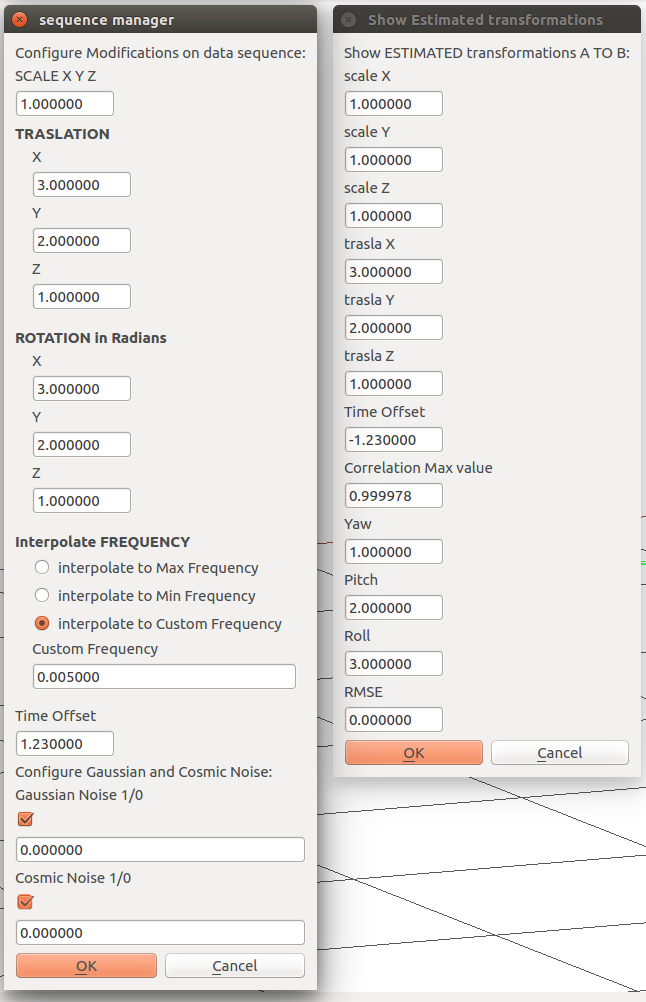
\includegraphics[height=16.0cm,width=12.0cm]{img/cap5/showTransformationsEstimated2.png}
\hspace{0.5cm}
\end{center}
\caption{Transformaciones realizadas frente Transformaciones estimadas }
\end{figure}


\begin{figure}[H]
\begin{center}
\label{fig:opciones de View}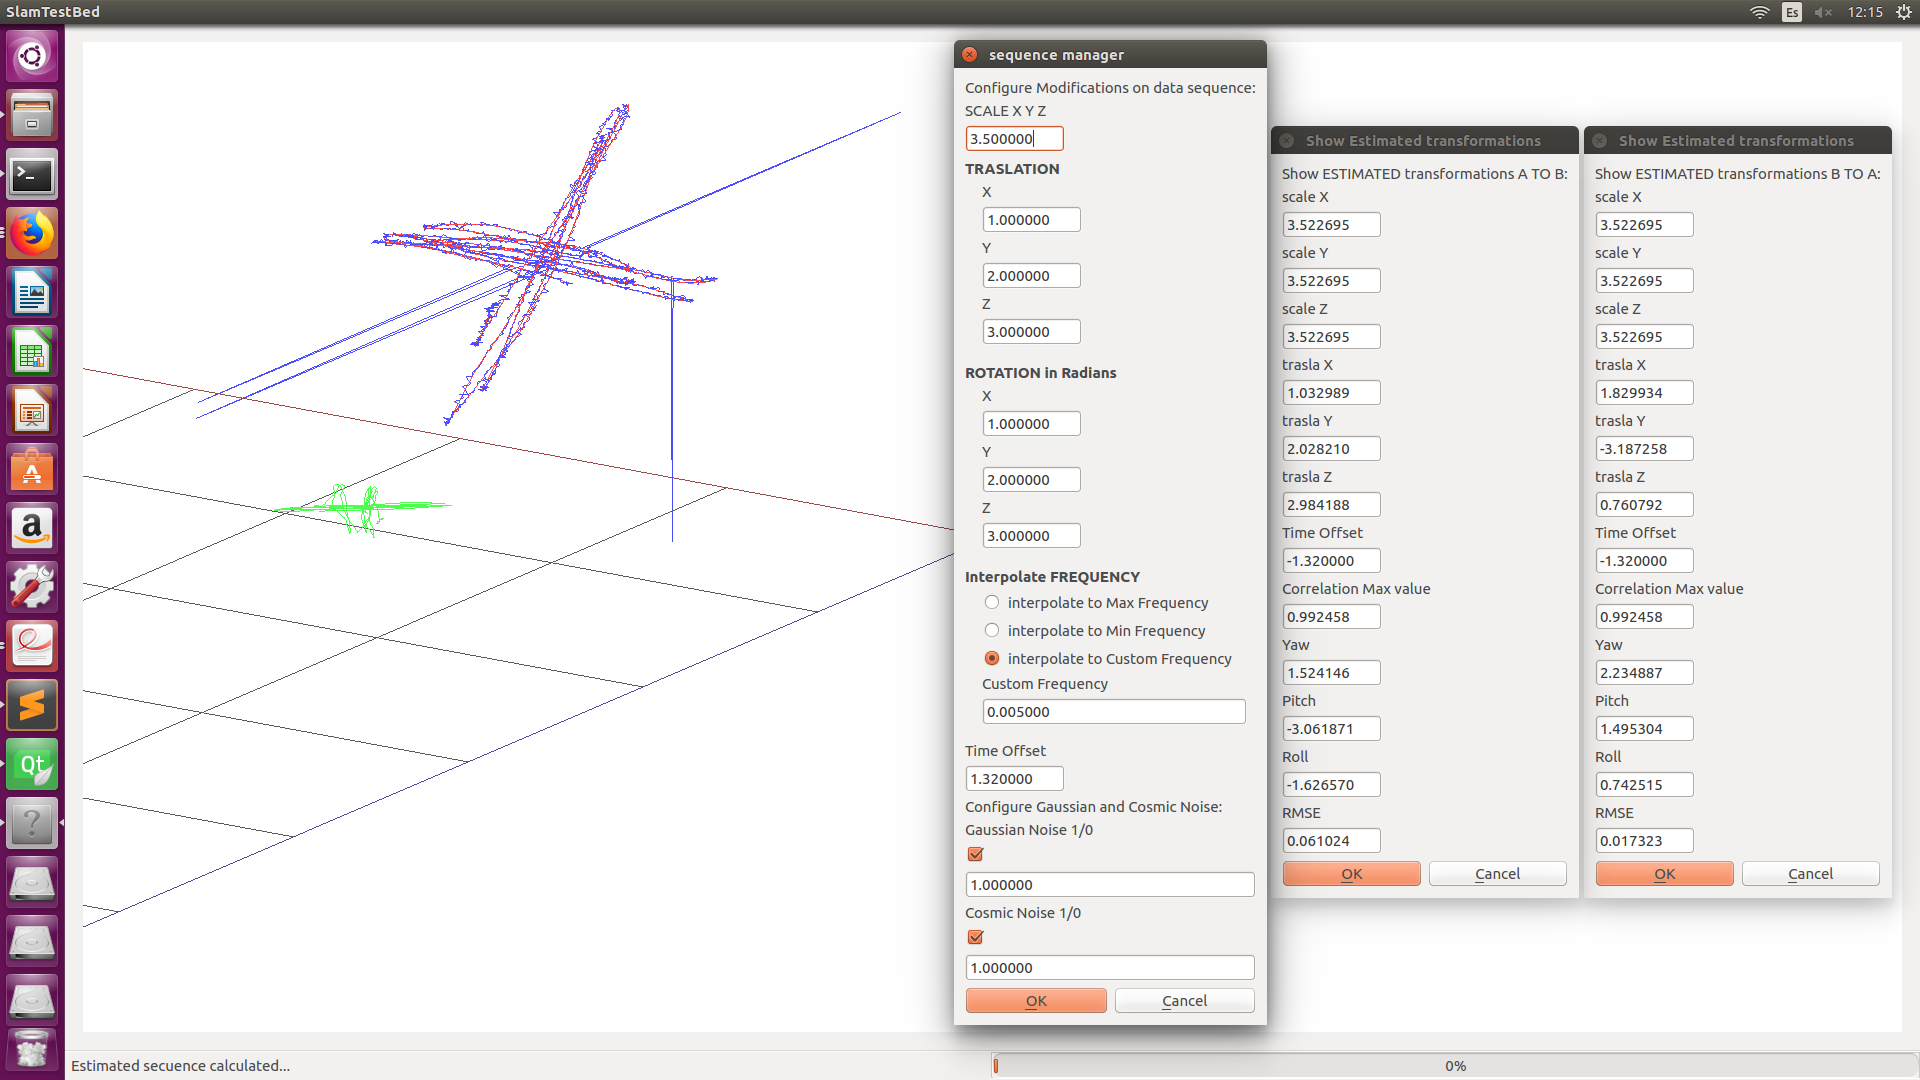
\includegraphics[height=12.0cm,width=17.0cm]{img/cap6/Escala_Trasla_Rota_Offset_Gauss_CosmicNoise_abba.png}
\hspace{0.5cm}

\end{center}

\caption{Resultados de la estimación de un cambio de escala y traslación .}
\end{figure}

En la interfaz gráfica podemos ver tres \textit{datasets}. Los puntos 3D del primer \textit{dataset} \textit{groundtruth} se pintarán en color verde, los puntos del \textit{dataset} a evaluar o \textit{dataset} transformado serán de color azul, y por último en color rojo estarán los puntos 3D del \textit{dataset} estimado.
En el caso de que el error entre los dos \textit{datasets} sea pequeño, los puntos 3D correspondientes al \textit{dataset} estimado solaparán con los puntos correspondientes a la verdad absoluta, lo que significará que la trayectoria calculada por el algoritmo de SLAM es cercana a la realidad y en este caso el punto estimado (en color rojo) quedará invisible. Además el GUI también muestra los valores de transformación estimadas (Figura 4.4)


%\clearpage

